%\begin{figure}[htb]
\begin{teaserfigure}
  \centering
  \subfloat[scene representation]{
    \label{fig:teaser:scene}
    % \includegraphics[height=4.5cm]{TOG/figs/scene.pdf}
    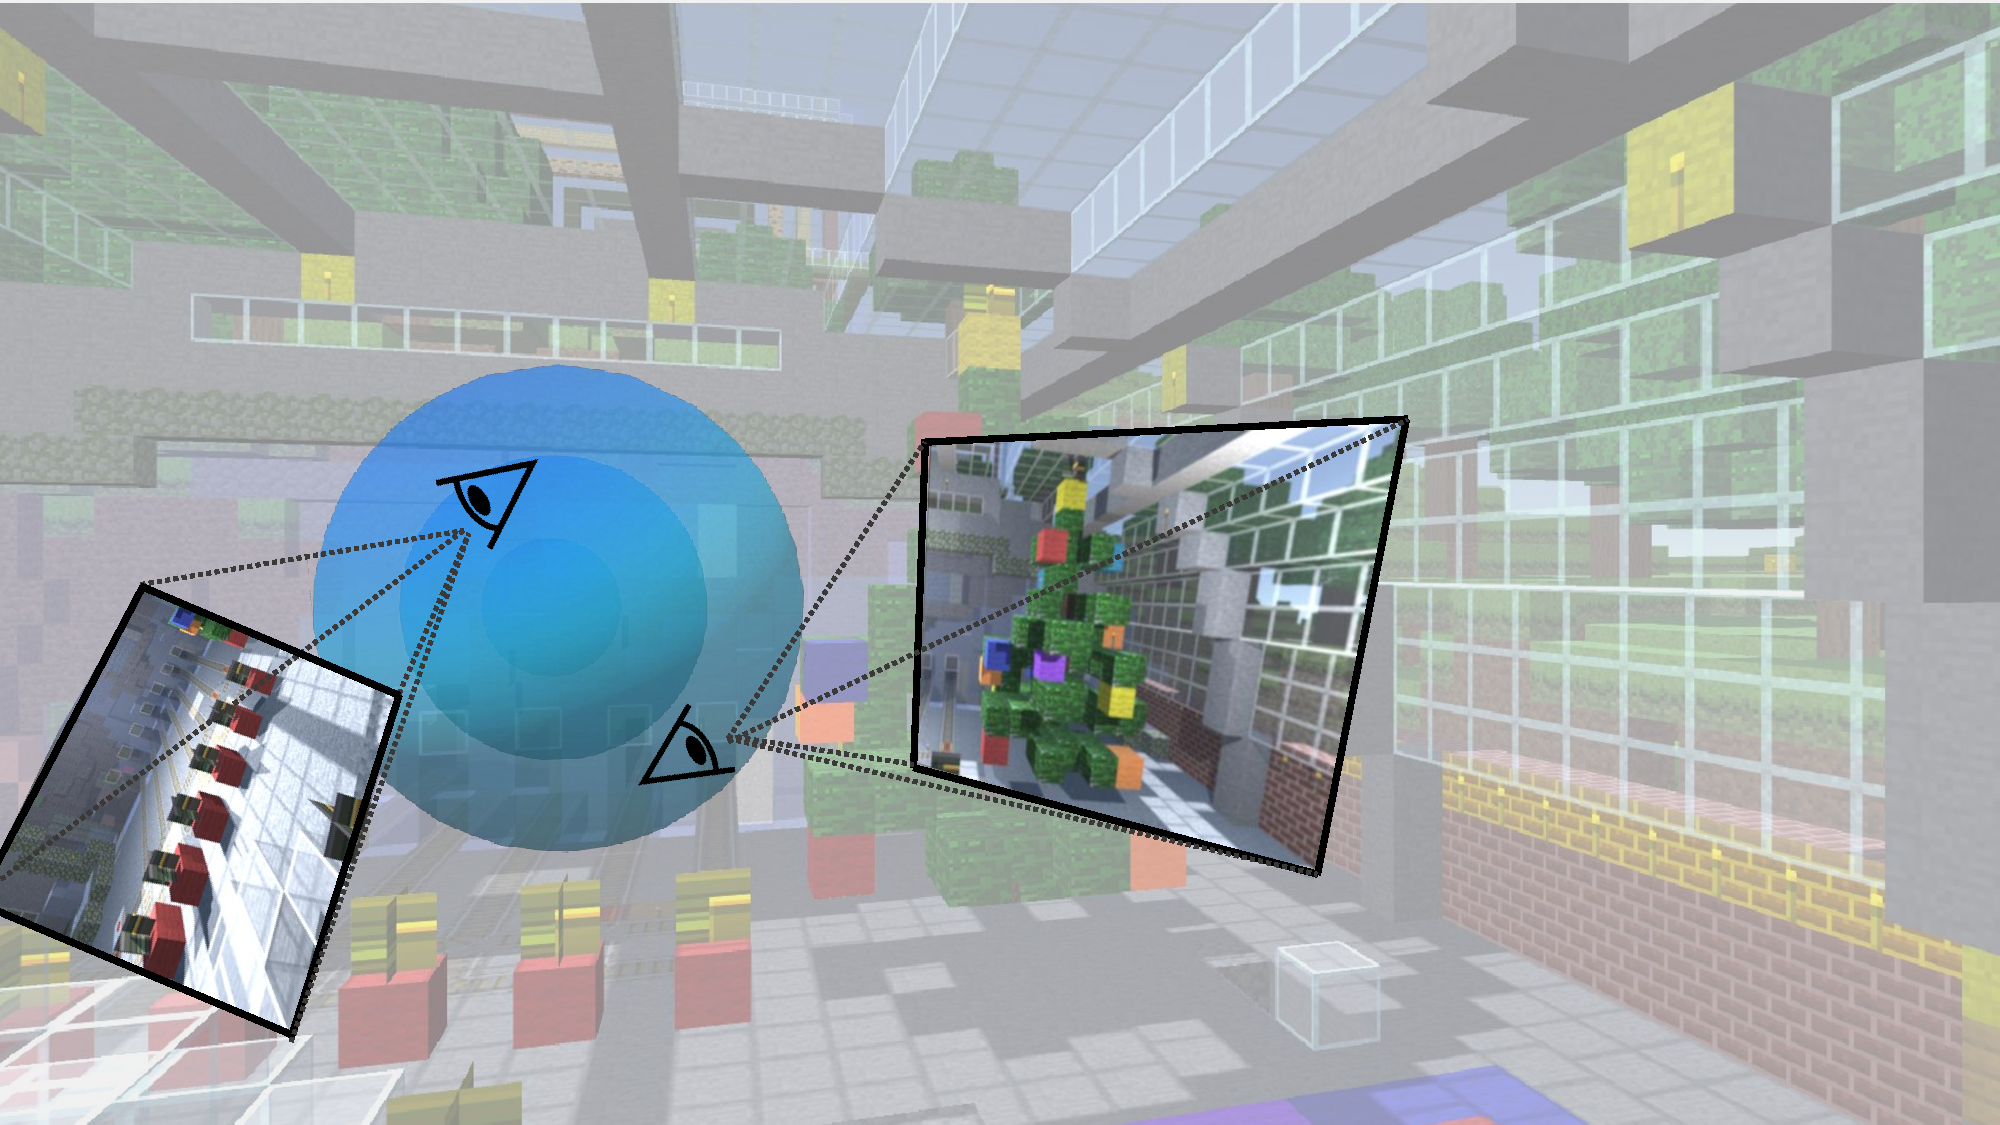
\includegraphics[height=4.5cm]{TOG/figs/teaser_1a_wc.pdf} %try other colors a little bit
  }%subfloat
  \subfloat[latency]{
    \label{fig:teaser:latency}
    \includegraphics[height=4.5cm]{TOG/figs/teaser_1b_small.pdf}
    % \includegraphics[height=4.5cm]{TOG/figs/teaser.pdf}
    % nerf: 15+s/per infer
  }%subfloat
  \subfloat[foveal quality]{
    \label{fig:teaser:quality}
    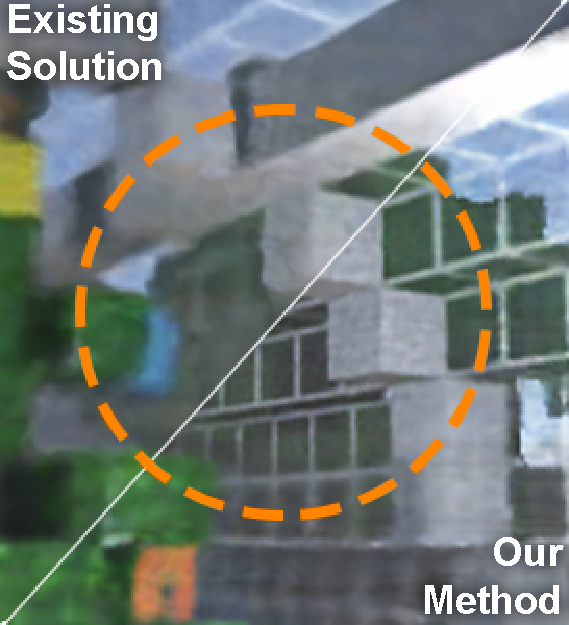
\includegraphics[height=4.5cm]{TOG/figs/teaser_1c.pdf}
  }%subfloat
 \Caption{Illustration of our system.}
 {% 
\subref{fig:teaser:scene} shows visualizes our active-viewing tailored scene representation.
Comparing with \protect\cite{mildenhall2020nerf}, \subref{fig:teaser:latency} shows our benefits of reduced latency.
As a zoom-in, \subref{fig:teaser:quality} compares our foveal quality preservation.
\qisun{Cross out half-half in  \subref{fig:teaser:latency}. TODO for myself: I should make the background scene semi-transparent. Will do so soon.}
 }
 \label{fig:teaser}
%\end{figure}
\end{teaserfigure}
